\subsection{Peking}

Comencemos por describir la ruta generada(Ver mapa que todavía no está). Se han realizado 29 saltos hasta alcanzar el destino solicitado, de los cuales, aproximadamente en el $86 \% $ de los mismos, hemos obtenido respuestas del tipo $TIME\_EXCEEDED$, determinando así, que el largo de nuestra ruta es de 25 saltos, y que del resto de los valores del $TTL$ no hemos obtenido respuesta alguna. Como también se puede ver en el (mapa que no está), durante el trayecto se realizaron 3 saltos intercontinentales, correspondientes a los hops 9, 10 Y 20.

% MAPAS ACA

Analicemos ahora los outliers detectados por Cimbala y contrastemos los datos con la realidad.

\begin{table}[!htbp]
\centering
\caption{Traceroute Peking}
\label{traceroute-peking}
\begin{tabular}{|c|c|c|c|c|c|}
\hline
\textbf{TTL} & \textbf{IP}     & \textbf{RTT} & \textbf{STANDARIZED RTT} & \textbf{COUNTRY} & \textbf{OUTLIERS} \\ \hline
1            & 10.0.2.2        & 0.672730     & 0.352331                 & Undefined        &                   \\ \hline
6            & 200.89.161.149  & 17.053374    & 0.085501                 & Argentina        & {[}outlier{]}     \\ \hline
7            & 200.89.165.130  & 0.000000     & 0.370312                 & Argentina        &                   \\ \hline
8            & 200.89.165.222  & 1.996175     & 0.316957                 & Argentina        &                   \\ \hline
9            & 185.70.203.32   & 0.000000     & 0.370312                 & Italy            &                   \\ \hline
10           & 89.221.41.181   & 132.068054   & 3.159685                 & United States    & {[}outlier{]}     \\ \hline
11           & 89.221.41.181   & 2.382882     & 0.306621                 & United States    &                   \\ \hline
12           & 154.54.9.17     & 11.118905    & 0.073119                 & United States    & {[}outlier{]}     \\ \hline
13           & 154.54.80.41    & 0.000000     & 0.370312                 & United States    &                   \\ \hline
14           & 66.28.4.237     & 14.763109    & 0.024286                 & United States    & {[}outlier{]}     \\ \hline
15           & 154.54.29.222   & 7.872963     & 0.159878                 & United States    & {[}outlier{]}     \\ \hline
16           & 154.54.42.77    & 0.831040     & 0.348099                 & United States    &                   \\ \hline
17           & 154.54.45.162   & 2.006372     & 0.316684                 & United States    &                   \\ \hline
18           & 154.54.45.2     & 0.000000     & 0.370312                 & United States    &                   \\ \hline
19           & 38.88.196.186   & 0.815241     & 0.348522                 & United States    &                   \\ \hline
20           & 101.4.117.169   & 147.027389   & 3.559527                 & China            & {[}outlier{]}     \\ \hline
21           & 101.4.117.97    & 4.108167     & 0.260506                 & China            & {[}outlier{]}     \\ \hline
22           & 101.4.117.50    & 0.000000     & 0.370312                 & China            &                   \\ \hline
23           & 101.4.115.69    & 0.000000     & 0.370312                 & China            &                   \\ \hline
24           & 101.4.118.94    & 1.594142     & 0.327703                 & China            &                   \\ \hline
25           & 101.4.112.90    & 1.955545     & 0.318043                 & China            &                   \\ \hline
26           & 101.4.117.81    & 0.000000     & 0.370312                 & China            &                   \\ \hline
27           & 202.112.41.178  & 0.000000     & 0.370312                 & China            &                   \\ \hline
28           & 202.112.41.182  & 0.096631     & 0.367729                 & China            &                   \\ \hline
29           & 162.105.252.133 & 0.000000     & 0.370312                 & China            &                   \\ \hline
\end{tabular}
\end{table}


Como se puede observar en la tabla \ref{traceroute-peking}, el método propuesto por Cimbala ha determinado que existen 7 saltos cuyos tiempos son outliers. Como hemos mencionado previamente, tan solo se han producido 3 saltos entre continentes, dos de los cuales se han detectado correctamente, mientras que el noveno salto, entre Argentina e Italia, no ha sido identificado. Por lo tanto, podemos afirmar que el método ha presentado 5 casos de falsos positivos, es decir, casos que señaló como saltos intercontnentales y no lo eran, y un caso de falso negativo, donde no ha determinado que un salto sea entre continentes cuando si lo fue.

En cuanto al caso del falso negativo, es decir el salto entre Argentina e Italia, esto se debe a que el tiempo para ese hop fue 0, con lo cual, el mismo pudo haber sido efectivamente 0 o más bien un valor negativo que hemos reemplazado con un cero. Este valor, que ya lo hemos visto en el experimento de otra universidad, puede deberse a algunos de los factores que hemos planteado al principio del presente documento en donde indicamos algunas hipótesis del por qué de tiempos negativos. \\
Más allá de eso, cabe mencionar que, si el tiempo que se corresponde con el salto es nulo, y que para la aplicación del método de Cimbala hemos decidido no contemplar los ceros, es claro que jamás lo iba a poder detectar como un outlier. Simplemente en esta ocasión el problema radicó en haber obtenido un tiempo negativo para dicho hop.


En las figura \ref{fig:10} y \ref{fig:11}, donde exponemos para cada salto su correspondiente tiempo y su valor estandarizado respectivamente, se puede observar como el $TTL$ 10 y 20 tienen un $RTT$ claramente distinguido del resto. 

En cuanto a los otros saltos detectados como outliers, más precisamente el 6, 12, 14 y 15, podemos decir que, visualmente, no parecen estar muy por encima del resto, por lo que entendemos que no deberían haber sido detectados como outliers, más allá de que tampoco han sido saltos intercontinentales.

\begin{figure}[!htbp]
  \centering
    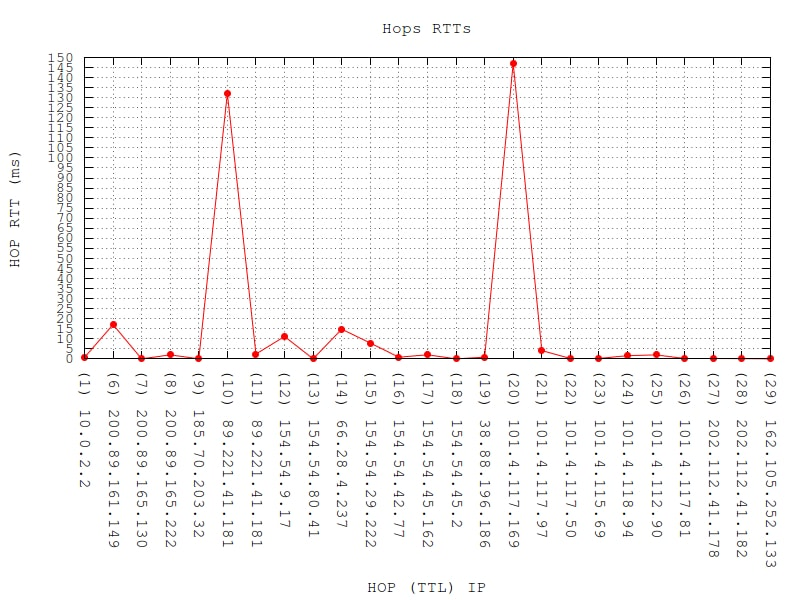
\includegraphics[scale=0.5]{imagenes/peking-graficos/traceroute-peking.jpg}
  \caption{peking- RTT hops}
  \label{fig:10}
\end{figure}


\begin{figure}[!htbp]
  \centering
    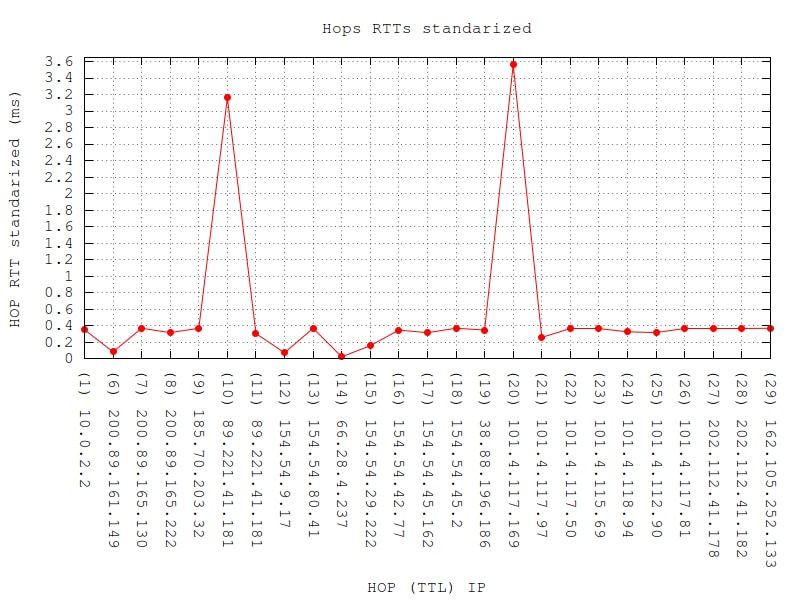
\includegraphics[scale=0.5]{imagenes/peking-graficos/traceroute-peking-standarized.jpg}
  \caption{peking- RTT hops standarized}
  \label{fig:11}
\end{figure}


